\section{Evaluation}

\begin{frame}
  \frametitle{Methodik}
  \begin{itemize}  
  	\item Verschiedene Szenarios
    \item Ein Default-Szenario: Übrige Szenarios sind Abwandlungen
    \item Jedes Szenario läuft 10 mal
    \item Plots: Durchschnitt und Konfidenzintervall (Konfidenzniveau 95\%)
  \end{itemize}	
\end{frame}



\begin{frame}
  \frametitle{Methodik}
  \begin{block}{Besonderheiten}
    \begin{itemize}
      \item Verbindungen nur virtuell: Kein TCP
      \vspace{2mm}
      \item Keine (De-)Serialisierung von Paketen: Spart CPU und RAM
      \vspace{2mm}
      \item Aber: Paketgröße wird simuliert!
    \end{itemize}
  \end{block}
\end{frame}


%%%
%%% DEFAULT SCENARIO 1
%%%

\begin{frame}
  \frametitle{Default Szenario}
  \begin{block}{Einstellungen}
	  \begin{itemize}  
	    \item 1 Super-Peer und 63 Peers
	    \item Doppelt so viele Chunks wie Peers (126 Chunks)
	    \item Gleiche Uploadbandbreite für Super-Peer und Peers
	    \item Datengröße so gewählt, dass $T_0=10$ Minuten gilt 
	  \end{itemize}		
  \end{block}
\end{frame}


\begin{frame}
  \frametitle{Default Szenario - Completion}
  \begin{itemize}  
    \item Links: Ablauf des Datentransfers
    \item Rechts: Peers absteigend sortiert nach Gesamtdauer
  \end{itemize}

  \begin{center}
    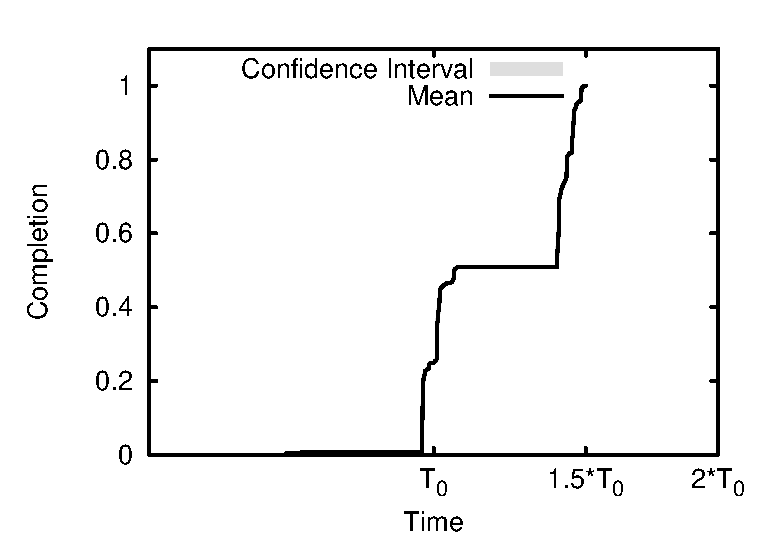
\includegraphics[width=0.49\textwidth]{fig/plots/scenario_1_default/plots/GeneratedMeanChunkCompletion.csv.eps}
    \hfill
    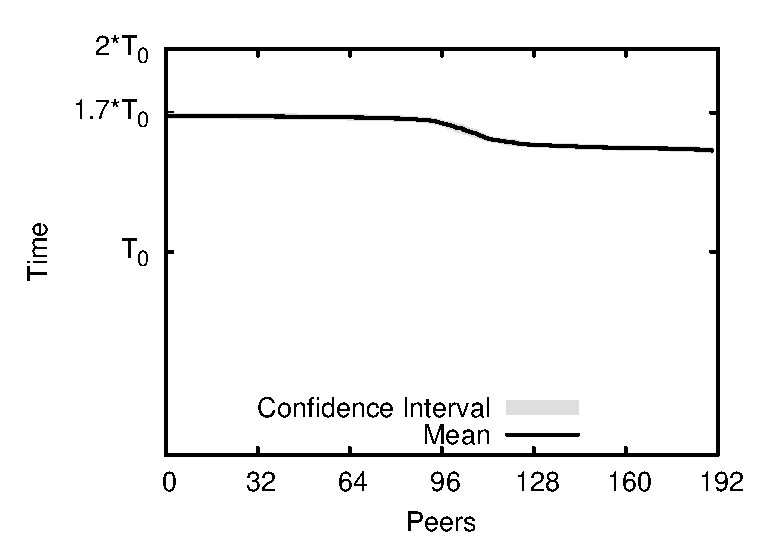
\includegraphics[width=0.49\textwidth]{fig/plots/scenario_1_default/plots/GeneratedMeanSortedChunkCompletion.csv.eps}
  \end{center}
\end{frame}


\begin{frame}
  \frametitle{Default Szenario - Upload/Download}
  \begin{center}
    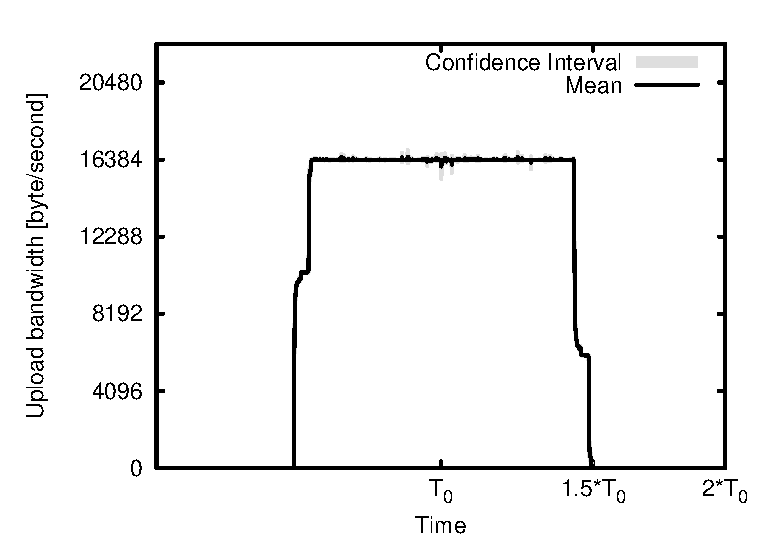
\includegraphics[width=0.49\textwidth]{fig/plots/scenario_1_default/plots/GeneratedMeanCurrentUploadBandwidth.csv.eps}
    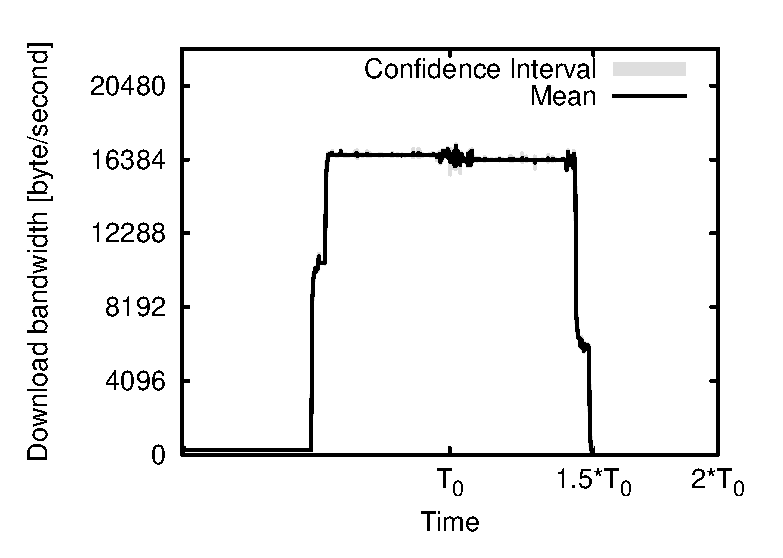
\includegraphics[width=0.49\textwidth]{fig/plots/scenario_1_default/plots/GeneratedMeanCurrentDownloadBandwidth.csv.eps}
  \end{center}
\end{frame}


\begin{frame}
  \frametitle{Default Szenario - Super-Peer Upload}
  \begin{center}
    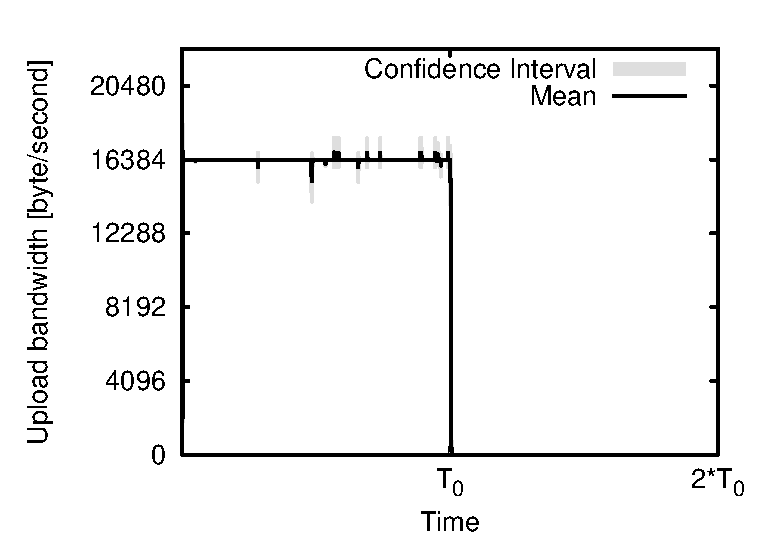
\includegraphics[width=0.49\textwidth]{fig/plots/scenario_1_default/plots/GeneratedMeanCurrentSuperSeederUploadBandwidth.csv.eps}
  \end{center}
\end{frame}


%%%
%%% SCENARIO 128
%%%

\begin{frame}
  \frametitle{Ergebnisse - Default Szenario mit 128 Peers}
  Completion Graph:
  
  \begin{center}
    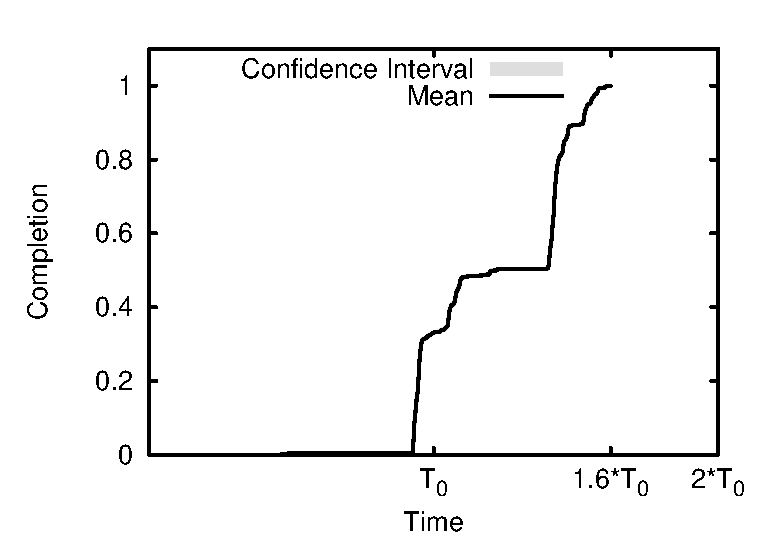
\includegraphics[width=1\textwidth]{fig/plots/scenario_4_peer_count_128/plots/GeneratedMeanChunkCompletion.csv.eps}
  \end{center}
\end{frame}


\begin{frame}
  \frametitle{Ergebnisse - Default Szenario mit 128 Peers}
  Super-Peer Upload Bandwidth:
  
  \begin{center}
    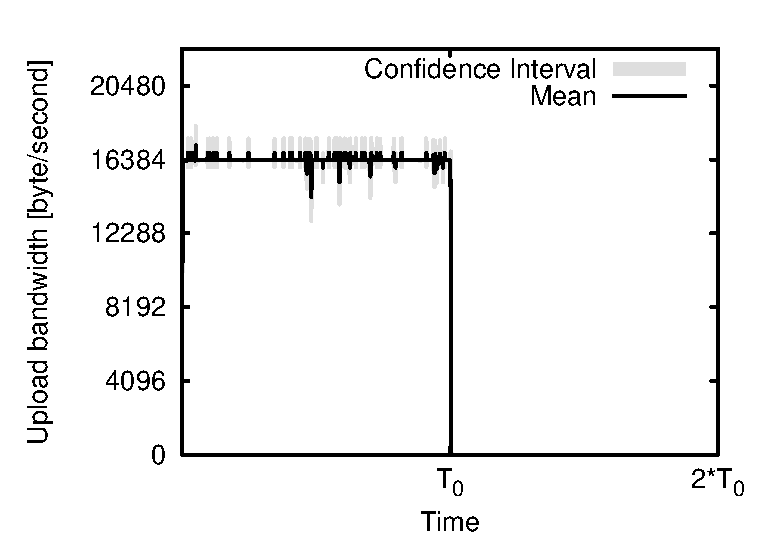
\includegraphics[width=1\textwidth]{fig/plots/scenario_4_peer_count_128/plots/GeneratedMeanCurrentSuperSeederUploadBandwidth.csv.eps}
  \end{center}
\end{frame}


\begin{frame}
  \frametitle{Ergebnisse - Default Szenario mit 128 Peers}
  Peer Upload Bandwidth:
  
  \begin{center}
    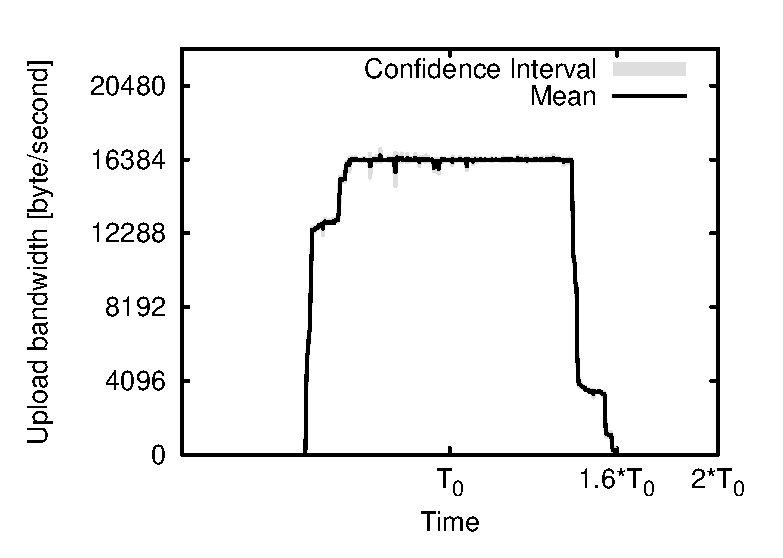
\includegraphics[width=1\textwidth]{fig/plots/scenario_4_peer_count_128/plots/GeneratedMeanCurrentUploadBandwidth.csv.eps}
  \end{center}
\end{frame}


\begin{frame}
  \frametitle{Ergebnisse - Default Szenario mit 128 Peers}
  Peer Download Bandwidth:
  
  \begin{center}
    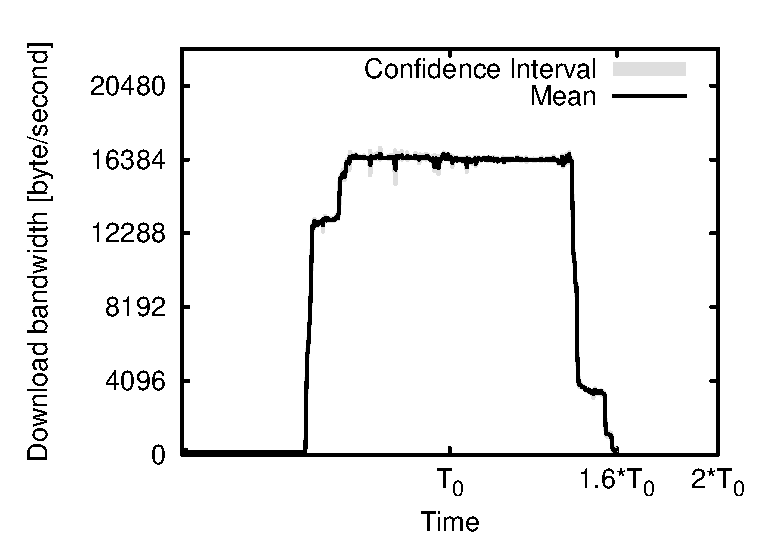
\includegraphics[width=1\textwidth]{fig/plots/scenario_4_peer_count_128/plots/GeneratedMeanCurrentDownloadBandwidth.csv.eps}
  \end{center}
\end{frame}

%%%
%%% SCENARIO 192
%%%

\begin{frame}
  \frametitle{Ergebnisse - Default Szenario mit 192 Peers}
  Completion Graph:
  
  \begin{center}
    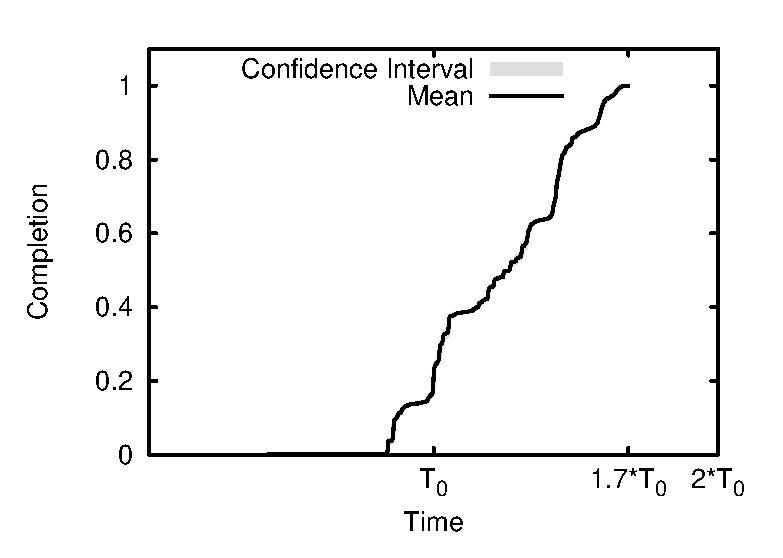
\includegraphics[width=1\textwidth]{fig/plots/scenario_11_peer_count_192_v2/plots/GeneratedMeanChunkCompletion.csv.eps}
  \end{center}
\end{frame}


\begin{frame}
  \frametitle{Ergebnisse - Default Szenario mit 192 Peers}
  Super-Peer Upload Bandwidth:
  
  \begin{center}
    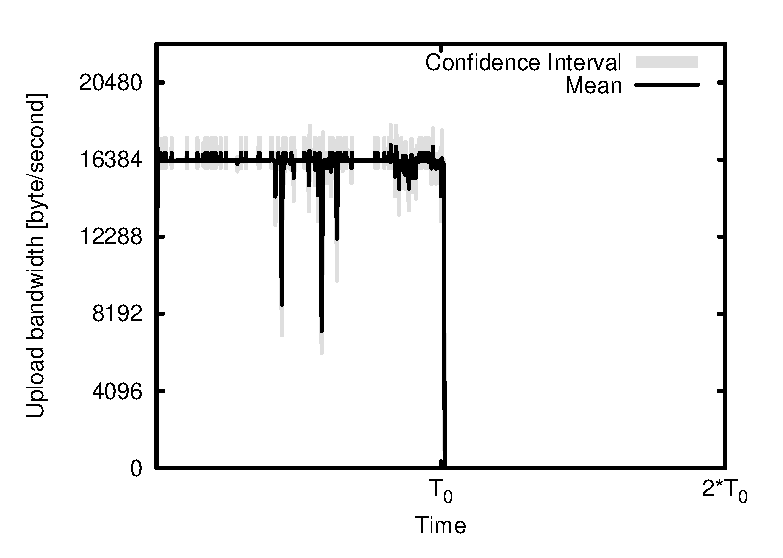
\includegraphics[width=1\textwidth]{fig/plots/scenario_11_peer_count_192_v2/plots/GeneratedMeanCurrentSuperSeederUploadBandwidth.csv.eps}
  \end{center}
\end{frame}


\begin{frame}
  \frametitle{Ergebnisse - Default Szenario mit 192 Peers}
  Peer Upload Bandwidth:
  
  \begin{center}
    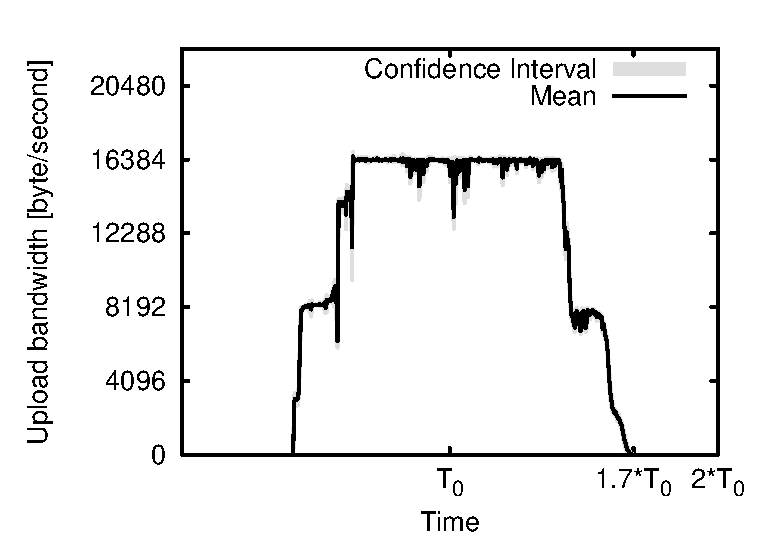
\includegraphics[width=1\textwidth]{fig/plots/scenario_11_peer_count_192_v2/plots/GeneratedMeanCurrentUploadBandwidth.csv.eps}
  \end{center}
\end{frame}


\begin{frame}
  \frametitle{Ergebnisse - Default Szenario mit 192 Peers}
  Peer Download Bandwidth:
  
  \begin{center}
    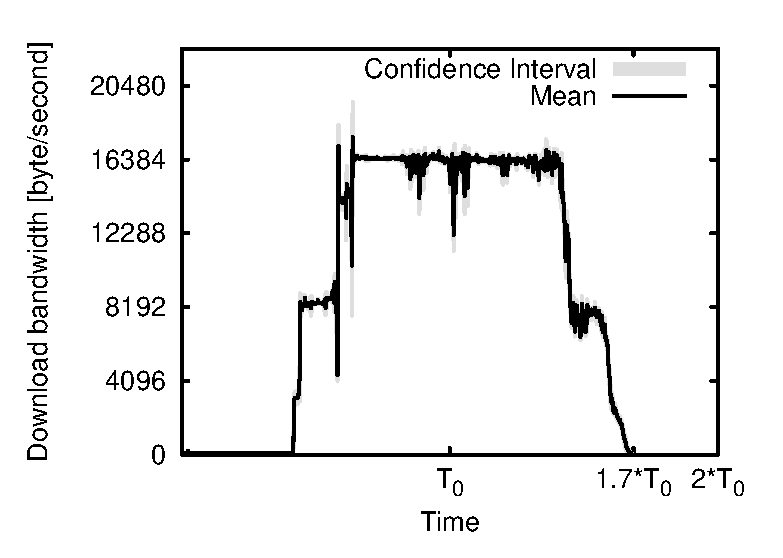
\includegraphics[width=1\textwidth]{fig/plots/scenario_11_peer_count_192_v2/plots/GeneratedMeanCurrentDownloadBandwidth.csv.eps}
  \end{center}
\end{frame}

%%%
%%% SCENARIO 4x Chunks
%%%

\begin{frame}
  \frametitle{Ergebnisse - Default Szenario mit 4x Chunkanzahl}
  Completion Graph:
  
  \begin{center}
    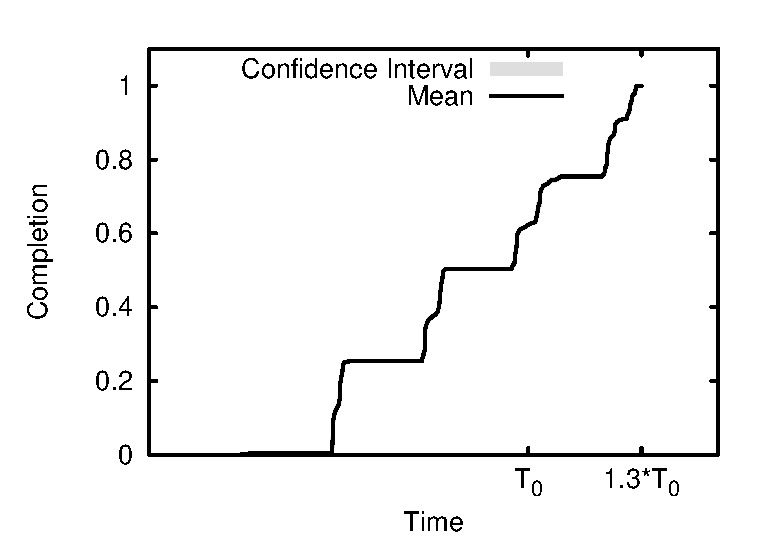
\includegraphics[width=1\textwidth]{fig/plots/scenario_15_chunk_count_fac_4/plots/GeneratedMeanChunkCompletion.csv.eps}
  \end{center}
\end{frame}


\begin{frame}
  \frametitle{Ergebnisse - Default Szenario mit 4x Chunkanzahl}
  Super-Peer Upload Bandwidth:
  
  \begin{center}
    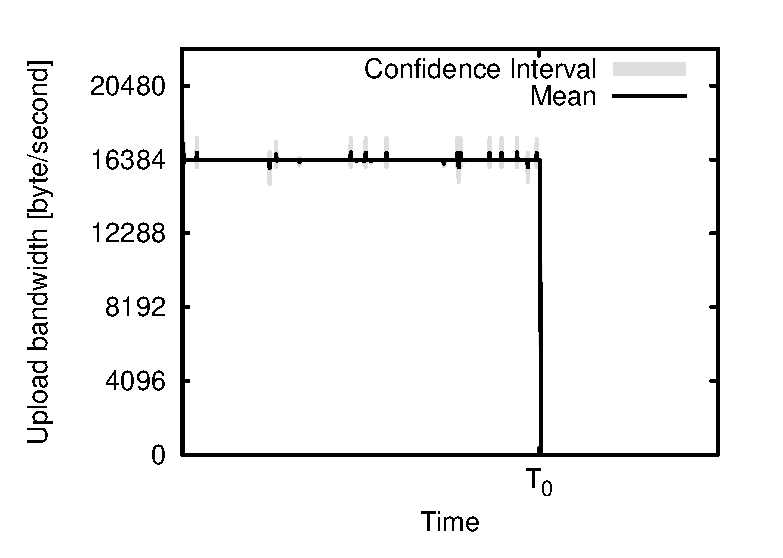
\includegraphics[width=1\textwidth]{fig/plots/scenario_15_chunk_count_fac_4/plots/GeneratedMeanCurrentSuperSeederUploadBandwidth.csv.eps}
  \end{center}
\end{frame}


\begin{frame}
  \frametitle{Ergebnisse - Default Szenario mit 4x Chunkanzahl}
  Peer Upload Bandwidth:
  
  \begin{center}
    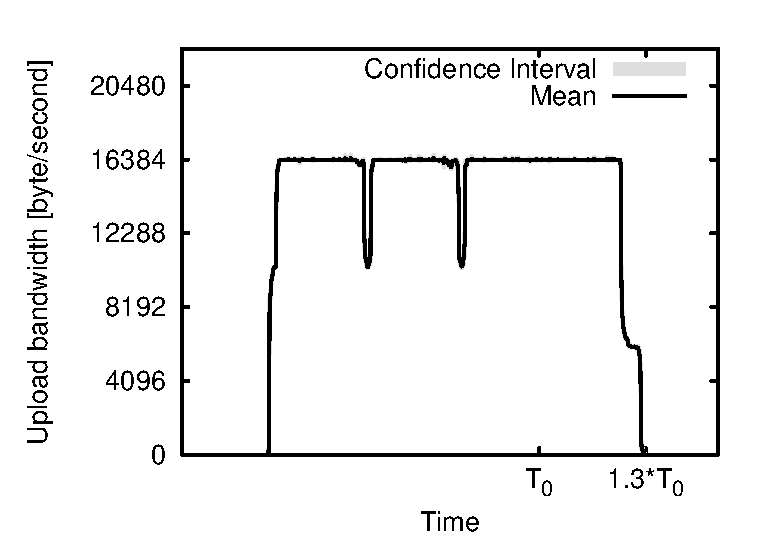
\includegraphics[width=1\textwidth]{fig/plots/scenario_15_chunk_count_fac_4/plots/GeneratedMeanCurrentUploadBandwidth.csv.eps}
  \end{center}
\end{frame}


\begin{frame}
  \frametitle{Ergebnisse - Default Szenario mit 4x Chunkanzahl}
  Peer Download Bandwidth:
  
  \begin{center}
    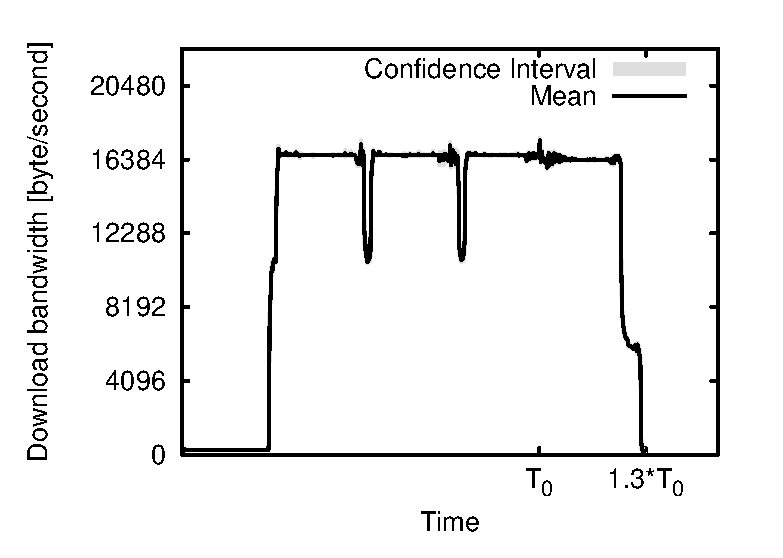
\includegraphics[width=1\textwidth]{fig/plots/scenario_15_chunk_count_fac_4/plots/GeneratedMeanCurrentDownloadBandwidth.csv.eps}
  \end{center}
\end{frame}



%%%
%%% SCENARIO Parts 20
%%%

\begin{frame}
  \frametitle{Ergebnisse - Default Szenario mit 20 Datensätzen (Stream)}
  Bislang gab es immer nur einen Datensatz, der verteilt wurde. Nun wird der gesamte Datensatz in 20 weitere Sub-Datensätze geteilt.

  \begin{itemize}  
    \item Jeder Sub-Datensatz hat wieder doppelt soviele Chunks wie Peers.
    \item Die Sub-Datensätze sind durchnummeriert mit IDs.
    \item Sub-Datensätze mit kleiner ID haben Vorrang.
    \item Streaming!
  \end{itemize}	
\end{frame}


\begin{frame}
  \frametitle{Ergebnisse - Default Szenario mit 20 Datensätzen (Stream)}
  Completion Graph:
  
  \begin{center}
    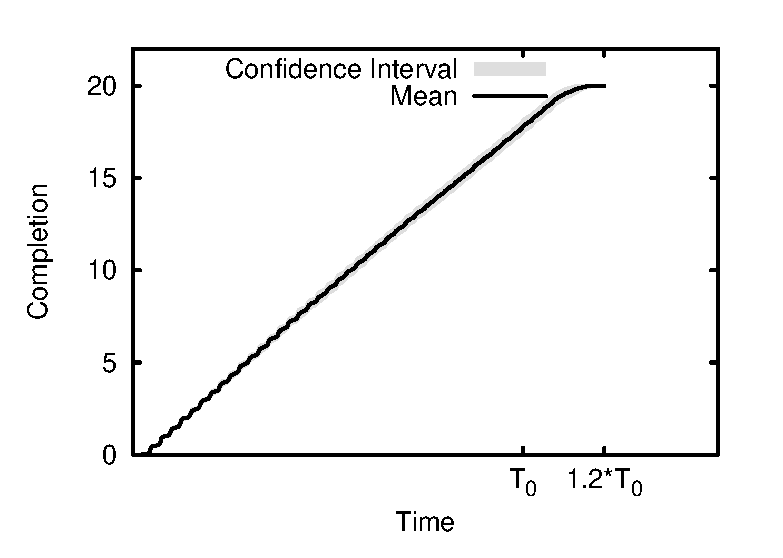
\includegraphics[width=1\textwidth]{fig/plots/scenario_6_parts_20/plots/GeneratedMeanChunkCompletion.csv.eps}
  \end{center}
\end{frame}


\begin{frame}
  \frametitle{Ergebnisse - Default Szenario mit 20 Datensätzen (Stream)}
  Super-Peer Upload Bandwidth:
  
  \begin{center}
    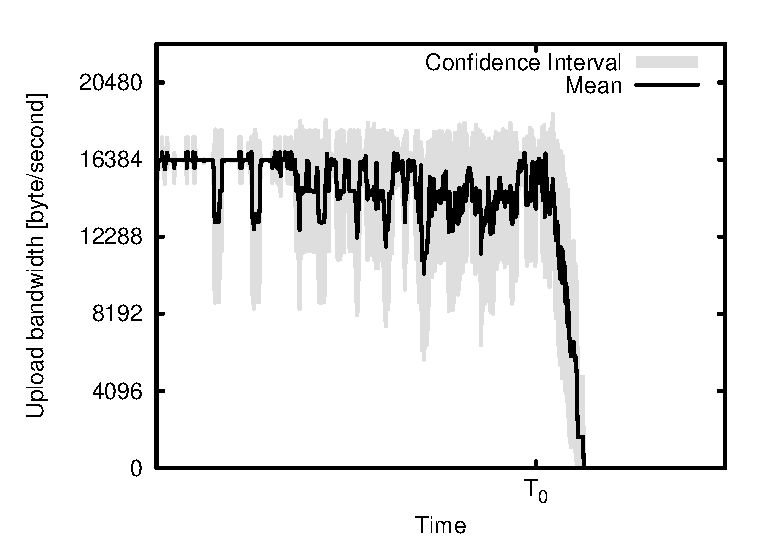
\includegraphics[width=1\textwidth]{fig/plots/scenario_6_parts_20/plots/GeneratedMeanCurrentSuperSeederUploadBandwidth.csv.eps}
  \end{center}
\end{frame}


\begin{frame}
  \frametitle{Ergebnisse - Default Szenario mit 20 Datensätzen (Stream)}
  Peer Upload Bandwidth:
  
  \begin{center}
    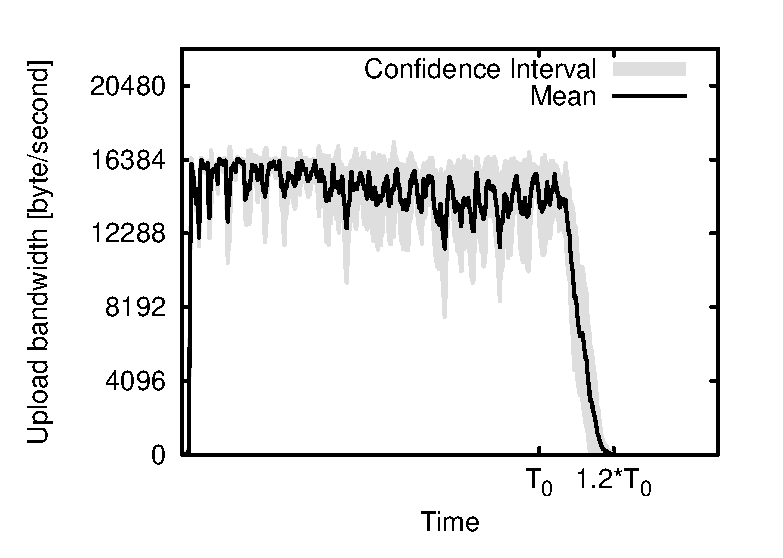
\includegraphics[width=1\textwidth]{fig/plots/scenario_6_parts_20/plots/GeneratedMeanCurrentUploadBandwidth.csv.eps}
  \end{center}
\end{frame}


\begin{frame}
  \frametitle{Ergebnisse - Default Szenario mit 20 Datensätzen (Stream)}
  Peer Download Bandwidth:
  
  \begin{center}
    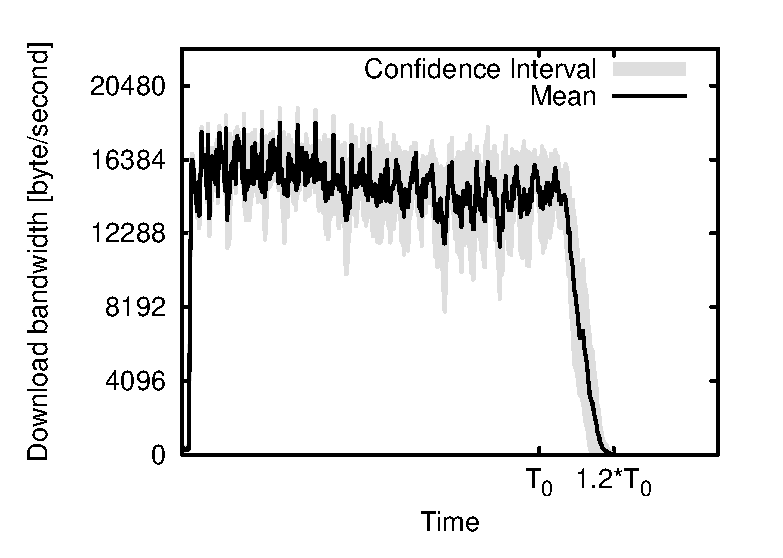
\includegraphics[width=1\textwidth]{fig/plots/scenario_6_parts_20/plots/GeneratedMeanCurrentDownloadBandwidth.csv.eps}
  \end{center}
\end{frame}





%%%
%%% SCENARIO Seq
%%%

\begin{frame}
  \frametitle{Ergebnisse - Szenario Sequential}
  Dieses Szenario implementiert zum Vergleich ein Client\,/\,Server System:

  \begin{itemize}  
    \item Es gibt einen Super-Peer (Server) und 63 Peers (Clienten).
    \item Die Peers sind nicht untereinander verbunden.
    \item Anzahl der Chunks spielt hier keine Rolle.    
    \item Datengröße so gewählt, dass $T_0=10$ Minuten gilt.
  \end{itemize}
\end{frame}

\begin{frame}
  \frametitle{Ergebnisse - Szenario Sequential}
  Completion Graph:
  
  \begin{center}
    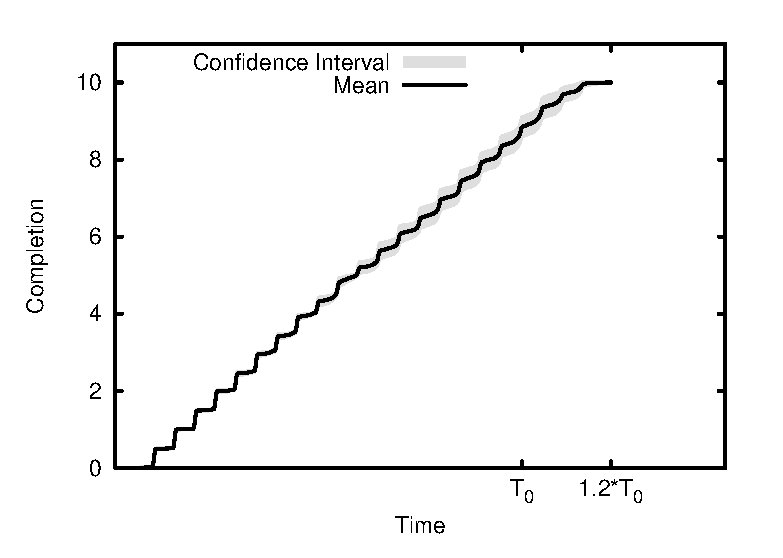
\includegraphics[width=1\textwidth]{fig/plots/scenario_2_seq/plots/GeneratedMeanChunkCompletion.csv.eps}
  \end{center}
\end{frame}

\begin{frame}
  \frametitle{Ergebnisse - Szenario Sequential}
  Super-Peer Upload Bandwidth:
  
  \begin{center}
    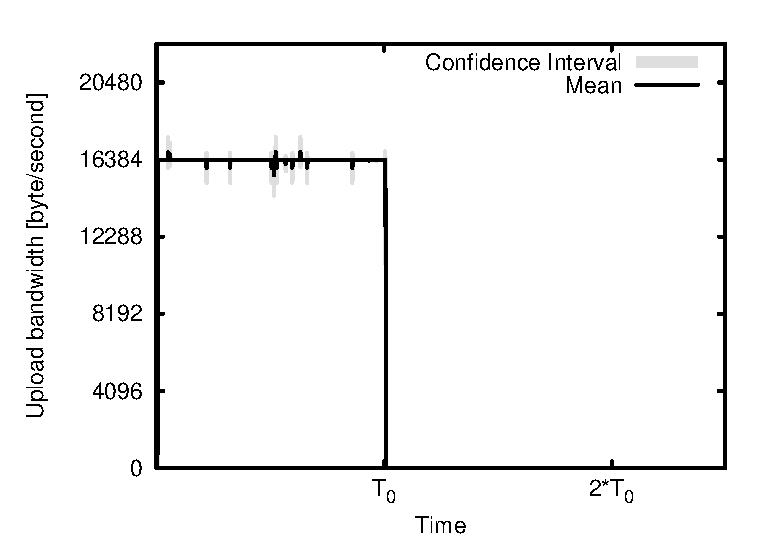
\includegraphics[width=1\textwidth]{fig/plots/scenario_2_seq/plots/GeneratedMeanCurrentSuperSeederUploadBandwidth.csv.eps}
  \end{center}
\end{frame}

\begin{frame}
  \frametitle{Ergebnisse - Szenario Sequential}
  Peer Download Bandwidth:
  
  \begin{center}
    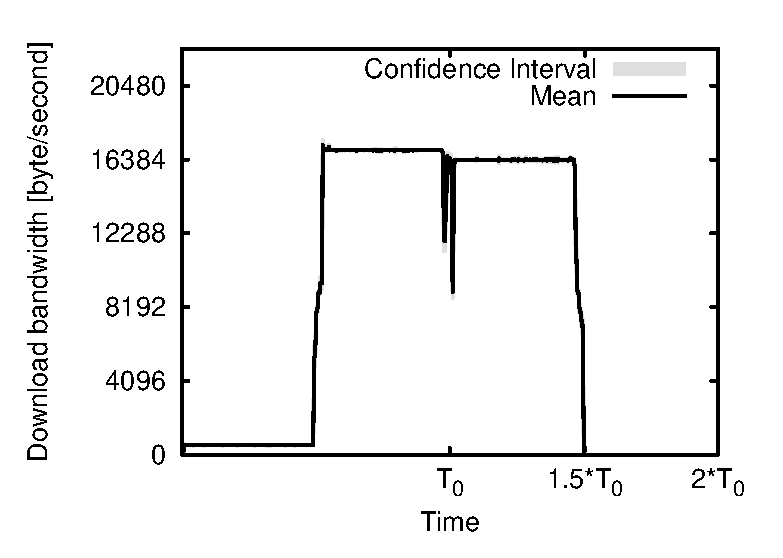
\includegraphics[width=1\textwidth]{fig/plots/scenario_2_seq/plots/GeneratedMeanCurrentDownloadBandwidth.csv.eps}
  \end{center}
\end{frame}


%%%
%%% Fazit
%%%

\begin{frame}
  \frametitle{Evaluation - Fazit}
  \setbeamertemplate{itemize items}[circle]
  \begin{itemize}
	  \item Mit Hilfe des Chunked-Swarm Verfahren kann man im Idealfall Lieferfristen weit unter $2*T_0$ garantieren, unabhängig von der Anzahl der Peers.
	  \item Die Anzahl der Peers sollte bekannt sein, um eine passende Anzahl an Chunks zu wählen.
	  \item Das System skaliert nicht endlos, da die Anzahl der Verbindungen quadratisch wächst.
	  \item Mit Hilfe von Sub-Datensätzen kann Streaming implementiert werden.
  \end{itemize}
\end{frame}

%%%
%%% Future Work
%%%

\begin{frame}
  \frametitle{Future Work}
  \setbeamertemplate{itemize items}[circle]
  \begin{itemize}
	  \item Einführung einer Simulationszeit, damit bei vielen Peers und sehr hoher CPU Auslastung die Messungen nicht beeinflusst werden.
	  \item Implementierung auf Basis eines Push-Based Ansatzes. Es gäbe keine Notwendigkeit mehr für Announcements.
	  \item Verwendung einer hierarchischen Struktur, um das Problem der quadratisch wachsenden Anzahl an Verbindungen zu verringern.
  \end{itemize}
\end{frame}
